\begin{figure}[tb]
    \centering
     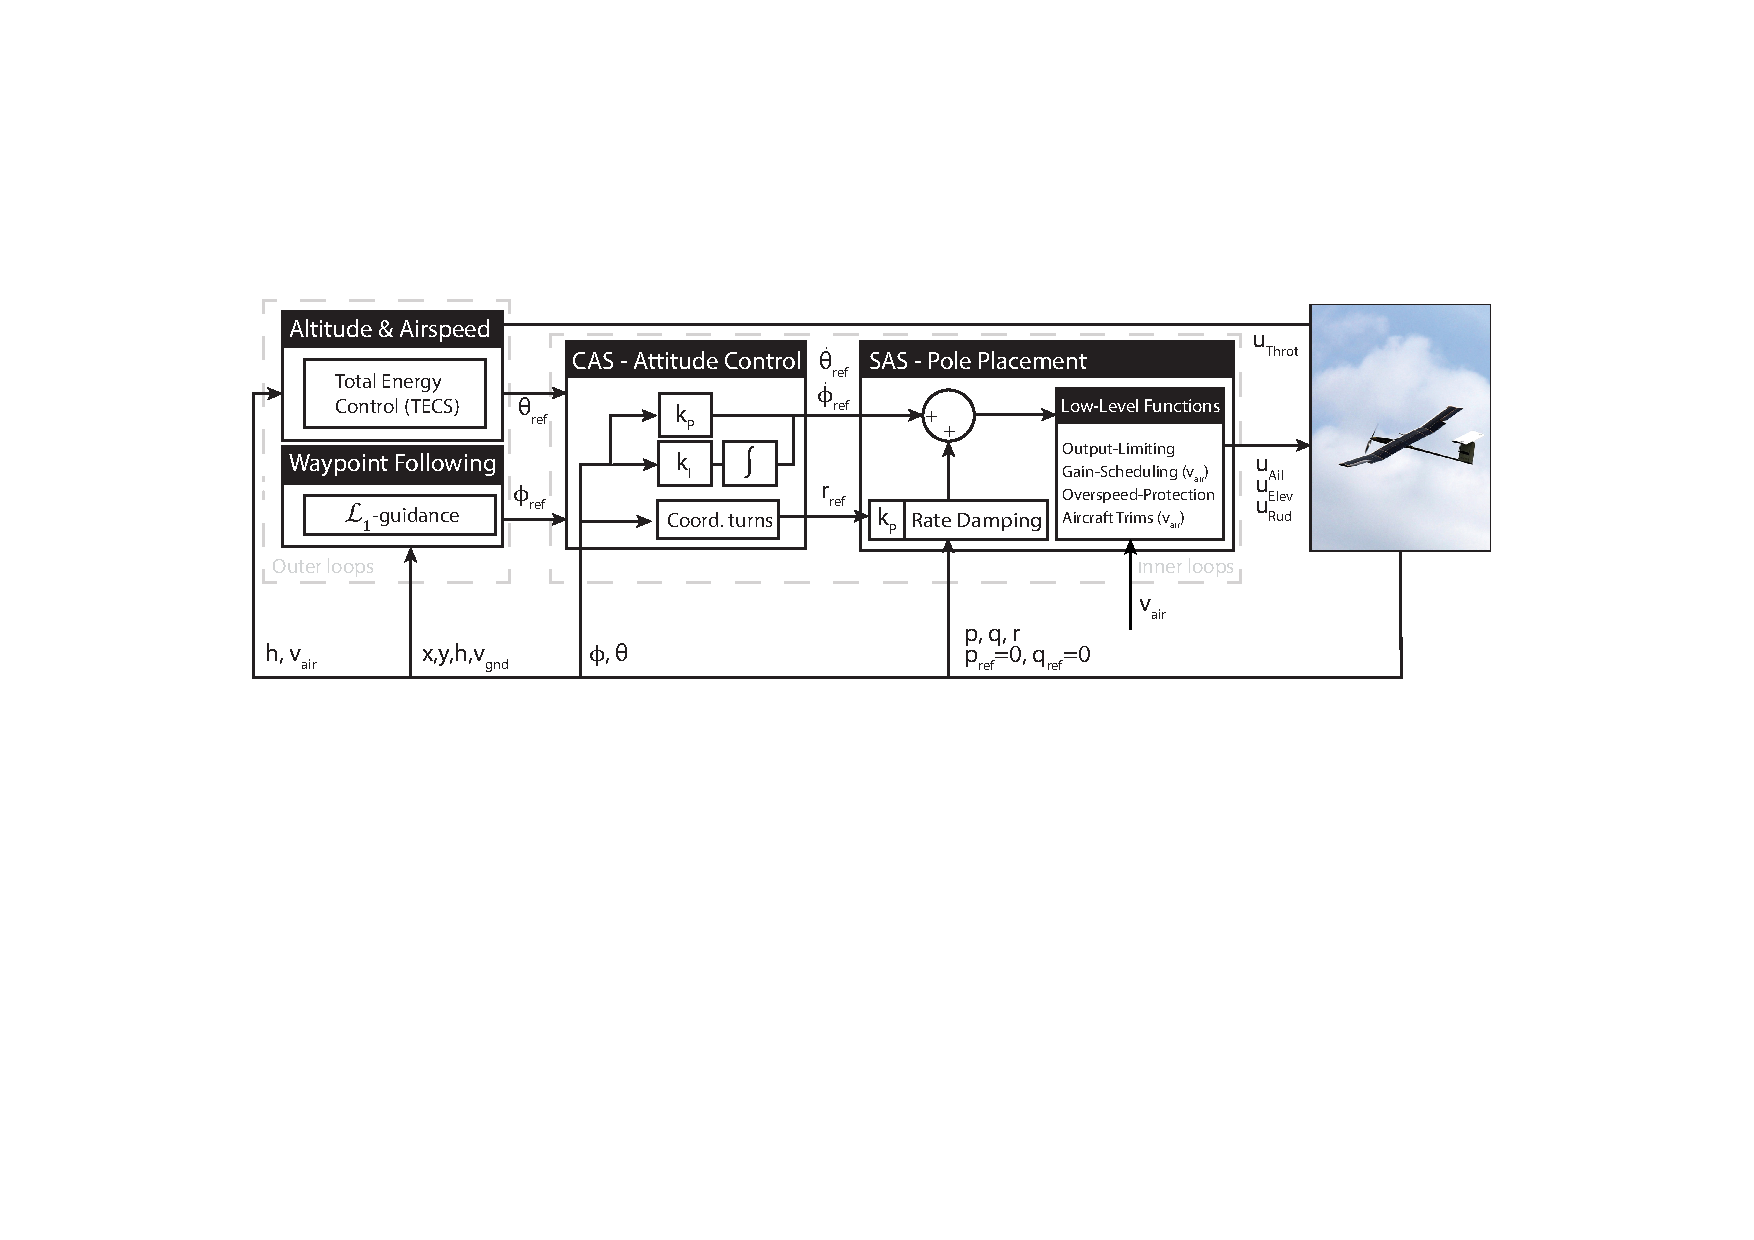
\includegraphics[width=\linewidth]{images/11_ControlScheme/ControlScheme.pdf}
    \caption{Control Scheme implemented for AtlantikSolar.}
    \label{fig:ControlScheme}
\end{figure}

AtlantikSolar features autonomous navigation up to the level of loitering through user--defined waypoints. The complete control structure (Fig.~\ref{fig:ControlScheme}) is offline tuned based on the identified system model (Sec.~\ref{sec:SystemID}), functionality is tested in an X--Plane 10 Hardware--In--the--Loop (HIL) simulation and finally refined in extensive flight tests. For inner--loop control, our baseline--solution corresponds to a set of cascaded saturated PID controllers: the Stability Augmentation System (SAS) applies rate--damping to shape the airplane's frequency response, while the Control Augmentation System (CAS) applies proportional--integral feedback to achieve roll ($\phi$) and pitch ($\theta$) reference tracking. Furthermore, flight tests showed that due to AtlantikSolar's high wingspan and thus high inertia ($I_z$ and $I_x$ especially), coordinated turn control is essential to smoothen the adverse yaw behaviour and achieve the no--sidelslip yaw rate $r=\frac{g\cdot \sin(\phi)}{v_{air}}$. To avoid overload of the highly optimized structure, output limiters are applied. Additionally, the control actions are in a final stage adapted with respect to the dynamic pressure $q=\frac{1}{2}\rho v^{2}_{air}$ which accounts for the change of the effective moments created by the control surfaces. 

Once the inner--loops are well--tuned, waypoint guidance is enabled. AtlantikSolar employs a $\pazocal{L}_1$--nonlinear guidance law which generates the lateral acceleration reference $a_{s_{ref}}$ and corresponding roll references $\phi_{ref}$ of the UAV based on a look--ahead distance ${L}_1$ and the current ground speed and heading as detailed in~\cite{HOW_L1nav} along with the online adaptation of the look--ahead distance as in~\cite{park2007performance}. This guidance law is integrated into our control structure as described in~\cite{Oettershagen_MED14_L1MPC} and combined with an extended version of the Pixhawk open--source Total Enery Control System (TECS)~\cite{PixhawkWebsite} which provides altitude control: First, a slew rate constraint on the reference altitude $h_{ref}$ has been integrated to reach smoother altitude control at pre-definable climb and sink rates, which is especially important for low propulsion-power to weight-ratio UAVs such as AtlantikSolar. Second, we've implemented ``thermal compliance'': In an updraft, the standard TECS implementation will decrease $\theta_{ref}$ to decrease the altitude if $h>h_{ref}$. To allow gaining potential energy from a thermal, we essentially make TECS use $\theta_{ref}$ fully and only for airspeed control and $u_{Throt}$ only for altitude control. When at $h>h_{ref}$, the plane will thus keep $\theta_{ref}=\theta_{ref}(t)$  such that $v(t)=v_{ref}(t)$ and will gradually disable the motor, potentially gaining altitude for strong thermals. Furthermore, hard constraints have been implemented, i.e. full throttle is forced for $h<h_{min}$, at $h>h_{max}$ we gradually allow a pitch-down and thus altitude decrease again, and at $h>h_{max}+50m$ the controller automatically engages the spoilers for maximum descend rate. The inner PID-based pitch- and roll control loops are executed at a sampling period of $T_{SAS,CAS}=0.01s$, while the high-level $\pazocal{L}_1$\&TECS controllers run with $T_{\pazocal{L}_1,TECS}=0.05s$. Given these settings, the full controller requires less than 4\% CPU load, 5KB of RAM and 47KB Flash memory and is thus computationally lightweight when compared to other Pixhawk applications (see~\cite{Oettershagen_MED14_L1MPC}) such as the state estimation. The whole controller is designed to be modular, and more sophisticated approaches like model predictive control~\cite{Oettershagen_MED14_L1MPC} and robust $H_\infty$--based controllers~\cite{Mosimann_FT} have been implemented and flown for evaluation on test planes in addition to the aforementioned PID--baseline inner--loop control solution. 